\NeedsTeXFormat{LaTeX2e}[2005/12/01]
%%    2010/04/06 v1.0 Vorlage Master-Forschungspraktikum Versuchsauswertung
%%    based on the 2009/10/14 v0.1 GAUBM template by Prof Pruschke

\documentclass[twoside,        %% zweiseitiges Layout
               BCOR12mm,       %% Bindekorrektur 12 mm
% please comment out if report is in English
               english,ngerman, %% Dokumentspr. Deutsch, Alternativspr. Englisch
% please remove comment if report is in English 
%               ngerman,english, %% Dokumentspr. Englisch, Alternativspr. Deutsch
               fleqn,headsepline=false,footsepline=false
              ]{Vorlage/MFPREPORT}
\makeatletter
\DeclareOldFontCommand{\rm}{\normalfont\rmfamily}{\mathrm}
\DeclareOldFontCommand{\sf}{\normalfont\sffamily}{\mathsf}
\DeclareOldFontCommand{\tt}{\normalfont\ttfamily}{\mathtt}
\DeclareOldFontCommand{\bf}{\normalfont\bfseries}{\mathbf}
\DeclareOldFontCommand{\it}{\normalfont\itshape}{\mathit}
\DeclareOldFontCommand{\sl}{\normalfont\slshape}{\@nomath\sl}
\DeclareOldFontCommand{\sc}{\normalfont\scshape}{\@nomath\sc}
\makeatother

%% Pakete und Definitionen ausgelagert
\input{Vorlage/packages}
\input{Vorlage/layout}

%% einbinden einiger nützlicher Befehle
\input{Vorlage/shortcuts}

%Zur Formatierung in der Matheumgebung
\renewcommand{\t}{\ensuremath{\rm\tiny}} % Tiefgestellter Text in der Matheumgebung wird schoener mit: $\Phi_{\t{Text}}$
\renewcommand{\d}{\ensuremath{\mathrm{d}}} % Die totale Ableitung ist stets aufrecht zu setzen: \d
\newcommand{\diff}[3][]{\ensuremath{\frac{\d^{#1}#2}{\d#3^{#1}}}} % einfache Ableitung nach x: $\ddx{\Phi}$
\newcommand{\pdiff}[3][]{\ensuremath{\frac{\partial^{#1}#2}{\partial#3^{#1}}}} % wie gesprochen, eine partielle Ableitung: \del
\newcommand{\aeqiv}{\ensuremath{\qquad \Longleftrightarrow \qquad}} % Eine Aequivalenz
\newcommand{\folgt}{\ensuremath{\qquad \Longrightarrow \qquad}} % Ein Folgepfeil mit Abstaenden
\newcommand{\corresponds}{\ensuremath{\mathrel{\widehat{=}}}} % Befehl für "Entspricht"-Zeichen
\newcommand{\mi}[1]{\ensuremath{\mathit{#1}}} % italics für griechische Buchstaben in Matheumgebung

%Um nicht so viel schreiben zu müssen...
\newcommand{\bs}[1]{\boldsymbol{#1}}
\newcommand{\ol}[1]{\overline{#1}}
\newcommand{\wtilde}[1]{\widetilde{#1}}
\newcommand{\mrm}[1]{\mathrm{#1}}
\newcommand{\mbf}[1]{\mathbf{#1}}
\newcommand{\mbb}[1]{\mathbb{#1}}
\newcommand{\mcal}[1]{\mathcal{#1}}
\newcommand{\mfrak}[1]{\mathfrak{#1}}

%Abkürzungen
\newcommand{\zB}{z.\,B.\ }
\newcommand{\bzw}{b.\,z.\, w.\ }
\newcommand{\Dh}{d.\,h.\ }
\newcommand{\Gl}{Gl.\ }
\newcommand{\Abb}{Abb.\ }
\newcommand{\Tab}{Tab.\ }

\usepackage{cleveref}
\usepackage{braket}


\begin{document}
\LabratoryName{FM.ULP}{Spatial and Temporal Distortion of Ultrashort Light Pulses}
\ProtocolAuthor{Eric}{Bertok}{eric.bertok@stud.uni-goettingen.de}
\Assistant{Dr. Sabine}{Steil}
\ResearchFocus{Festkörper- und Materialphysik (M.phy.403)}
% In der naechsten Version beruecksichtigt
%\Collaborator{Vorname}{Nachname}{email}
\ConductedOn{22}{11}{2017}
\date{\today}
% eines von beiden
\CopyNotWanted
%\CopyWanted

\pagenumbering{roman}
\maketitle

%\begin{otherlanguage}{english}
%\end{otherlanguage}

\tableofcontents

\clearpage
\pagenumbering{arabic}

\section{Einleitung}
\label{sec:einleitung}
\section{Theorie}
\label{sec:theorie}
\subsection{Grundlagen}
Zur Beschreibung Ultrakurzer Laserpulse verwendet man einen semiklassischen
Ansatz, bei dem die Maxwell-Gleichungen für eine makroskopische Polarisation
gelöst wird. Im Folgenden wird das Vektorfeld des elektrischen Feldes $\vec E$
durch einen Skalar $E$ genähert [Diels]. Hiermit wird eine für das Experiment
relevante Polarisationsrichtung beachtet. Im Allgemeinen sind auch Effekte
möglich, bei denen verschiedene Polarisationsrichtungen miteinander koppeln,
was eine genauere Betrachtung erfordert.
Ausgehend von dem elektrischen Feld $E(t)$ definiert man mithilfe der Fourier
Transformation das komplexe Spektrum
$\tilde{E}(\omega)=\mathcal{F}[E(t)]=\int_\mathbb{R}E(t)e^{-i\omega t}\d t
\label{eq:FT}$.
Die Rücktransformation ergibt sich zu $E(t)=\mathcal{F}^{-1}[\tilde
E(\omega)]=\frac{1}{2\pi}\int_{\mathbb R}\tilde E(\omega)e^{i\omega t}\d
\omega$. Dies funktioniert aufgrund der Linearität der Maxwell Gleichungen. Die
Lösung kann somit in eine Superposition von ebenen Wellen zerlegt werden. Hier
ist $\omega$ die Kreisfrequenz der ebenen Welle. Nach konvention wird häufig
nur der positive Anteil des Spektrums betrachtet. Er hat aufgrund der
Reellwertigkeit von $E$ den vollen Informationsgehalt
[Diels]. Bei der Fourier-Rücktransformation integriert man so nur über alle
positiven $\omega$ [Diels].
Ein Puls wird nun beschrieben durch [Trebino lec]
\begin{align}
    E(t)=\frac{1}{2}\sqrt{I(t)}\exp\left(i\left[ \omega _0 t-\Phi(t)
    \right]\right),
    \label{eq:efield}
\end{align}
wobei $\omega_0$ die sog. Trägerfrequenz und $\phi(t)$ eine allgemeine Phase in
Abhängigkeit von der Zeit $t$ ist. Die Trägerfrequenz ist der oszillatorische
Anteil des Pulses innerhalb der Einhüllenden $\sqrt{I(t)}$ und wird häufig in
eine komplexe Einhüllende $E_0$ integriert. Die Phase $\phi(t)$ beschreibt die
Zeitliche Veränderung der Farbe des Pulses. $I(t)=|E(t)|^2$ ist die
Intensität des Pulses. Ist $I$ eine stark gepeakte Funktion, so redet man von
einem ``ultrakurzen Puls''. Analog kann man durch $S=|\tilde E(\omega)|^2$ die
spektrale Intensität einführen. Somit gilt $\tilde
E(\omega)=\sqrt{S(\omega)}\exp(-i\varphi(\omega))\label{eq:spectrum}$, wobei
$\varphi(\omega)$ die spektrale Phase ist. Diese ist zentrale Größe bei der 
Beschreibung von gechirpten Pulsen (siehe unten).
Die Beschreibung des Spektrums ist auch mithilfe der Wellelänge $\lambda$
möglich. Die Umrechnung ergibt sich zu [Trebino lec]:
\begin{align}
    S_\lambda(\lambda)=S_\omega\left(\frac{2\pi c}{\lambda^2}\right)\frac{2\pi
    c}{\lambda^2}.
    \label{eq:lambdaspec}
\end{align}


\subsection{Instantane Frequenz und Chirp}
Die instantane Frequenz eines ultrakurzen Pulses ist definiert als [trebino lec]
\begin{align}
    \omega_{\text{inst}}=\omega_0-\diff{\phi}{t},
    \label{eq:instfrequ}
\end{align}
mit der Phase $\phi$ und der Trägerfrequenz $\omega_0$. Man kann nun sowohl die Phase, als auch die spektrale Phase taylorentwickeln: 
\begin{align}
    \phi(t)&=\phi_0+\underbrace{\diff{\phi}{t}|_{t=0}}_{\phi_1}t+\underbrace{\diff[2]{\phi}{t}|_{t=0}}_{\phi_2}\frac{t^2}{2}+\cdots,\\
    \varphi(w)&=\varphi_0+\underbrace{\diff{\varphi}{\omega}|_{\omega=\omega_0}}_{\varphi_1}(\omega-\omega_0)+\underbrace{\diff[2]{\varphi}{\omega}|_{\omega=\omega_0}}_{\varphi_2}\frac{(\omega-\omega_0)^2}{2}+\cdots.
    \label{eq:taylor}
\end{align}
Hier ist $\varphi_1=\diff{\varphi}{\omega}|_{\omega=\omega_0}$ der sogenannte
``group delay''(GD) und
$\varphi_2=\diff[2]{\varphi}{\omega}|_{\omega=\omega_0}$ die ``group delay
dispersion (GDD). Hieraus ist zu sehen: Eine nichtverschwindendes $\phi_1$
erzeugt nach \cref{eq:instfrequ} einen konstanten offset in der instantenen
Frequenz. Dies resultiert nach dem Fourier shift theorem [CITE] zu einer
Verschiebung im Spektrum. Andersherum erzeugt ein nicht verschwindender GD
einen offset in der temporalen Intensität. Dies ist zur bestimmung von
Pulslängen irrelevant. Ist jedoch $\varphi_2$ ungleich Null, so kommt es zur
Dispersion: Die Gruppengeschwindigkeit ändert sich für verschiedene Frequenzen
unterschiedlich und der Puls verläuft. Einen solchen Puls nennt man (linear) gechirpt. Analoges passiert bei einem nichtverschwindenden $\phi_2$. Die instantane Frequenz ändert sich hier linear mit der Zeit.

\subsection{Gaußpuls und Bandprodukt}
\label{seq:bandprod}
Die am einfachst zu handhabene Pulsform ist die eines Gaußpulses: [DIELS]
\begin{align}
    E(t)=E_0\exp\left[-2\ln 2\left(\frac{t}{\tau_{\text{FWHM}}}\right)\right].
    \label{eq:gaus}
\end{align}
$\tau_{\text{FWHM}}$ bezeichnet die ``full-width half maximum'', also die Halbwertsbreite des Pulses, welche eine von vielen Definitionen zur Beschreibung der Puls- oder Spektralbreite ist. Sie ist definiert als die Breite an der Halben Pulshöhe. Im Folgenden wird stets $\tau\equiv\tau_{\text{FWHM}}$ gesetzt. Der Gaußpuls ist neben seiner einfachen Handhabbarkeit auch eine der am häufigsten auftretenden Pulsformen.\\
Da (Kreis-) Frequenz und Zeit konjugierte Variablen einer Fourier Transformation sind, gilt für sie die Unschärferelation, genannt ``Zeit-Bandbreiteprodukt'': [Diels]
\begin{align}
    \braket{\omega^{2}}\braket{t^{2}} \geq \frac{M^{4}}{4}\kappa_c,
    \label{eq:time-bandwidth}
\end{align}
wobei $\braket{\Delta\omega^{2}}$ bzw $\braket{\Delta t^{2}}$ die Pulsbreite bzw die Bandbreite -berechnet durch das zweite Moment [Diels]- bezeichnet. $M$ ist ein Formfaktor, der die Abweichung zum idealen Gaußpuls bezeichnet [CITE]. $\kappa_c$ ist der Chirpfaktor, welcher angibt, dass bei gechirpten Pulsen das Zeit-Bandbreiteprodukt größer ist, als für ungechirpte Pulse. Einen ungechirpten Puls bezeichnet man demnach auch als ``Fourier-limitiert''. Fourier-limitierte Pulse sind also für eine konstante Bandbreite stets am kürzesten.
Die Umrechnung von den zweiten Momenten zur Halbwertsbreite ist für Gaußpulse
einfach über die Varianz einer Gaußverteilung zu berechnen. Es gilt
$\tau=2\sqrt{2 \ln 2}\braket{t^2}$. Aus \cref{eq:time-bandwidth} mit $M=1$ und
$\kappa_c=1$ lässt sich ebenfalls $\braket{\omega^2}=\frac{1}{4 \braket{t^2}}$
durch die Halbwertsbreite ausdrücken. Ausgedrückt durch die reguläre Frequenz
$\nu$
erhält man
\begin{align}
    \label{eq:bandprodeasy}
    \Delta \nu \Delta t = 0.441.
\end{align}

\subsection{Dispersion im Medium}
Bewegt sich ein Lichtpuls durch ein Medium, so wird eine Transferfunktion im Frequenzbild zum elektrischen Feld multipliziert [trebino lec]: $\tilde E_{\text{out}}(\omega)=\tilde{E}_{\text{in}}(\omega)\exp(-\alpha(\omega)L)\exp(-i n(\omega)k_0L)$. Hier beschreibt $\alpha$ die Absorption, welche in diesem Versuch ignoriert wird. $n(\omega)$ ist der Brechungsindex des Materials in Abhängigkeit von der Frequenz, $k_0$ ist die Wellenzahl bei der Trägerfrequenz und $L$ ist die Länge des Materials. Relevant für die Verbreiterung von Pulslängen ist die Modulation der spektralen Phase. Aufgrund der Form der Transferfunktion wird diese direkt hinzuaddiert [trebino]:
\begin{align}
    \varphi_{\text{out}}(\omega)=\varphi_{\text{in}}+n(\omega)k_0L.
    \label{eq:transferphase}
\end{align}
Eine Taylornäherung des Wellenvektors $k(\omega)=n(\omega)k_0$ ergibt analog zu \cref{eq:taylor} die sog. ``group velocity dispersion'' (GVD): [TREBINO]
\begin{align}
    \text{GVD}=k''(\omega_0)=\frac{1}{2}\frac{\lambda_0^3}{2\pi c_0^2}\diff[2]{n}{\lambda},
    \label{eq:gvd}
\end{align}
mit der Trägerwellenlänge $\lambda_0$ und der Lichtgeschwindigkeit $c_0$.
Es gilt GDD $=$ GVD $ L$.
Der wellenlängenabhängige Brechungsindex berechnet sich aus der Sellmeier Gleichung [CITE refr.]:
\begin{align}
    n^2(\lambda)=\frac{B_1 \lambda^2}{\lambda^2-C_1}+\frac{B_2 \lambda^2}{\lambda^2-C_2}+\frac{B_3 \lambda^2}{\lambda^2-C_3},
    \label{eq:sellmeier}
\end{align}
mit materialspezifischen numerischen Konstanten $B_i, C_i$, die z.B. in
\cite{refr} aufgelistet sind.\\
Für die Veränderung der Pulsbreite in Abhängigkeit der GDD gilt folgende
Beziehung, die in dieser Version durch Wigner-Distributionen [DIELS]
hergeleitet wird:
\begin{align}
    \braket{t^2}=\braket{t_0^2}+\left[ \diff[2]{\varphi}{\omega}|_{0}
    \right]^2\braket{\omega^2},
    \label{eq:pulsverbreiterung}
\end{align}
der Chirp, den der Puls erfährt berechnet sich also durch ``GDD $\times$
Bandbreite''. Aus den Umrechnungsregeln in \cref{seq:bandprod} kann man somit
den Effekt von einer group velocity dispersion auf einen Puls mit gegebener
Bandbreite berechnen.
\section{Experimentelle Methoden und Messgrößen}
\subsection{Spatial chirp}
Im Vergleich zu ebenen Wellen (continuous waves, cw's) bestehen ultrakurze
Pulse aus
sehr vielen Frequenzen: Sie haben eine hohe Bandbreite. Dies folgt unmittelbar
aus dem Fourierzusammenhang zwischen Bandbreite und Pulslänge, dem Bandprodukt
aus
\cref{eq:time-bandwidth}. Aufgrund dieser hohen Bandbreite sind ultrakurze
Laserpulse sehr viel anfälliger gegenüber Verzerrungen in der Zeit (temporaler
Chirp) und im Raum, da Dispersion stets durch einen veränderlichen
Brechungsindex in Abhängigkeit der verschiedenen Wellenlängen auftritt.
Zeitliche Verzerrungen sorgen für eine Pulsverbreiterung nach
\cref{eq:time-bandwidth}. Ein analoger Effekt tritt auch räumlich ein: Es kommt zu
einem räumlichen Chirp, wenn verschiedene Wellenlängen einen unterschiedlichen
Weg durch das Medium nehmen, wie zum Beispiel in einem Prismenkompressor
(s.u.). Anstatt zu verschiedenen Zeiten findet man hier die Farben des Pulses
an verschiedenen Orten, der Puls wird räumlich aufgefächert. Dieser Effekt
tritt durch Winkeldispersion, wie im Prismenkompressor, aber auch in einem
schrägen Glas ein, was in \cref{fig:spatialchirp} aufgezeigt ist.
\begin{figure}[]
    \centering
    \includegraphics[width=\textwidth]{spatialchirp.png}
    \caption{Spatial chirp verursacht durch einen Prismenkompressor (links) und
        ein schiefes Glas (rechts) \cite{tutspatialchirp}}
    \label{fig:spatialchirp}
\end{figure}
\subsection{Pulse front tilt}
Eine weitere räumliche Verzerrung ist der sog. Pulse front tilt. Er gibt an, um
wie viel die Pulsfront eines Laserpulses gegenüber der optischen Achse geneigt
ist. Er wird hervorgerufen durch Winkeldispersion oder auch durch das
Durchqueren eines räumlich gechirpten Pulses durch ein lineares Medium
(\cref{fig:pft}).
\begin{figure}[]
    \centering
    \includegraphics[width=0.5\textwidth]{pft.jpeg}
    \caption{Pulse front tilt verursacht durch Winkeldispersion (oben) und
        räumlichen Chirp (unten) \cite{Akturk:04}.}
    \label{fig:pft}
\end{figure}

\subsection{Prismenkrompressor}
\begin{figure}[]
    \centering
    \includegraphics[width=\textwidth]{pc.png}
    \caption{Schematischer Aufbau eines Prismenkompressors. Ein ungechirper
    Puls tritt ein und wird temporal gechirpt, da unterschiedliche Wellenlängen
    andere Propagationspfade nehmen. Bei entgegengesetztem Durchgang wird
    ersichtlich: Ein gechirpter Puls wird durch einen Prismenkompressor bei
    richtiger Einstellung ungechirpt, ``komprimiert''. Die Insertion ist definiert als der
    Abstand des Eintrittspunktes der zentralen Wellenlänge (hier grün) und der
    Spitze des zweiten Prismas .\cite{wikipc}}
    \label{fig:pc}
\end{figure}
Mithilfe des Prismenkompressors (PC) kann ein gechirpter Puls wieder zu einem
(nahezu) fourierlimitierten Puls komprimiert werden. Der Aufbau des
Prismenkompressors ist in \cref{fig:pc} zu sehen. Der Puls durchquert zwei
Prismen, die entgegengesetzt parallel zueinander aufgestellt sind. Dabei sind
sie so positioniert, dass der Puls beim ersten Prisma gerade durch die Spitze
durchquert. Nach Snell's Gesetz verlassen die unterschiedlichen Wellenlängen
das erste Prisma in unterschiedlichen Winkeln. Dadurch durchqueren sie
unterschiedlich lange Strecken im zweiten Prisma. Durch die spezielle
Positionierung verlassen alle Wellenlängen das zweite Prisma wieder parallel,
aber mit einem räumlichen Chirp. Um diesen auszugleichen wird der Strahl an
einem spiegel zurückreflektiert und nimmt somit den gleichen Weg erneut durch
den Prismenkompressor. Durch die unterschiedlichen Weglängen der verschiedenen
Frequenzen kann bei richtiger Positionierung des zweiten Prismas die Group
Delay Dispersion negativ werden, wodurch ein gechirpter Puls entchirpt werden kann. Für die GDD des Prismenkompressors gilt: [DIELS]
\begin{align}
    \diff[2]{\varphi}{\omega}|_{\omega_0}=2\frac{\lambda_0^2}{2\pi c_0^2}\left[
    L_g\diff[2]{n}{\lambda}|_{\lambda_0}-(4L+\frac{L_g}{n(\lambda_0)^3})(\diff{n}{\lambda}|_{\lambda_0})^2
    \right],
    \label{eq:pc}
\end{align}
wobei $\lambda_0$ die Trägerwellenlänge, $L_g$ die Weglänge im Glas für die
Trägerwellenlänge und $L$ der Abstand der Spitzen der beiden Primsen ist. Für
symmetrisch positionierte Prismen in Brewsterwinkelkonfiguration gilt
$L_g=2I\frac{1}{\sqrt{1+n(\lambda_0)^2}}$ mit dem Einschub (insertion) des
zweiten Prismas $I$, welcher im Experiment mit der Millimeterschraube direkt
eingestellt wird.

\subsection{Grenouille}
Um einen zeitlichen Prozess zu messen, benötigt man einen zweiten kürzeren Prozess, um
den ersten auflösen zu können. Da ultrakurze Pulse einige Femtosekunden lang
sind, während die Elektronik auf der Nanosekundenskala agiert, ist es demnach
für solche besonders schwer, die Pulslänge zu messen. 
Es gibt verschiedene Methoden: Ein erste Ansatz ist es, mithilfe eines
Michelson-Interferrometers die Autokorrelation $A(\tau)=\int E(t)E^*(t-\tau)\d
t$ zu bestimmen. Aus der gemessenen Intensität lässt sich die grobe
Pulsstruktur rekonstruieren. Autokorrelationsmethoden haben allerdings viele
Probleme, wie die Unterschätzung der Pulslänge durch sog. kohärente Artefakte
\cite{swampintro}. Zusätzlich ist es unmöglich, die Phase eines ultrakurze
Pulses mithilfe dieser Methoden zu messen.

GRENOUILLE (Grating-eliminated No-nonsense Observation Of Ultrafast Incident
Laser Light E Fields) behebt alle Probleme von Autokorrelaionsmethoden und
liefert zusätzliche Informationen über den Puls: Es basiert auf dem ``Frequency
Resolved Optical Gating'' (FROG) [CITE FROG], bei dem die spektrale Intensität gegenüber
der zeitlichen Verzögerung des Auftreffens auf den Detektor , der sogenannte
Frog trace gemessen wird. Aus diesem wird mithilfe eines Algorithmus die
Pulsdauer, die Bandbreite sowie die Phase und die spektrale Phase
rekonstruiert. Bei GRENOUILLE wird ein vereinfachter Aufbau, bestehend aus
einem Fresnelschen Biprisma und einem second-harmonic generation (SHG) Kristall
verwendet. Der Aufbau und die Funktionsweise ist in \cref{fig:gren} zu sehen. Der breite SHG
Kristall fächert die unterschiedlichen Wellenlängen entlang einer Dimension
auf, während das Fresnelsche Biprisma in der anderen Dimension den Puls teilt
und mit unterschiedlicher Verzögerung mit sich selbst interferieren lässt.
Dadurch entsteht der Frog trace, welcher den Puls überestimiert. Somit lassen
sich alle relevanten Informationen eines ultrakurzen Pulses rekonstruieren
[CITE]. Insbesondere liefert die spektrale Phase den Chirp des Pulses. Es ist
jedoch darauf zu Achten, dass die Methode symmetrisch gegenüber der
Zeitrichtung ist und deswegen der Vorzeichen des Chirps nicht bestimmt wird.
Zusätzlich werden automatisch der pulse front tilt, sowie der räumliche Chirp
gemessen. Sie spiegeln sich im Frog trace jeweils als Verschiebung auf der
Verzögerungsachse und als Scherung des Traces wider.



\section{Durchführung}
\label{sec:durchfuehrung}
\subsection{Aufbau}
Der Versuchsafbau ist in \cref{fig:aufbau} zu sehen. Die verwendete Laserquelle
ist ein Spectra Physics Tsunami mit einer zentralen Wellenlänge von 800\;nm,
einer durchschnittsleistung von 400\;mW, einer Pulsrate von 76\;MHz und einer
Pulsdauer von 22\;fs bei einer Bandbreite von 58\;nm. Der Strahl durchquert
zunächst einer $\lambda/2$ Platte und wird p-polarisiert. Anschließend
durchquert er den Prismenkompressor. Der Abstand der Prismen von Spitze zu
Spitze wurde gemessen und beträgt $43,2\pm0.3$\;cm. Der Prismeneinschub wird
direkt über eine Millimeterschraube variiert. Dem Laser stehen nun
drei mögliche Strahlengänge zur Verfügung, welche jeweils mit Klappspiegeln
eingestellt werden können. Pfad 1 besteht aus metallischen Spiegeln und einer
optischen Bank, auf die verschiedene Glasfenster aus BK7 oder MgF2, sowie ein
Glasspat und ein Langpass Filter geschraubt werden können. Pfad 2 besteht aus
dielektrischen Spiegeln. Auf Pfad 3 durchquert der Strahl ein Spiegelpaar mit
jeweils 5 Reflektionen. Eshandelt sich hierbei um gechirpte Spiegel, was die
spätere Auswertung zeigt. Alle drei Pfade enden in dem Messinstrument, einem
Swamp Optics Grenouille (Modell 8-20-USB). Zur Justage der Strahlengänge stehen
diverse Justagespiegel, Infrarot-Irisblenden und Infrarotkarten bereit.

\begin{figure}[]
    \begin{center}
        \includegraphics[width=0.7\textwidth]{aufbau1.eps}
    \end{center}
    \caption{Versuchsaufbau. Der Laser passiert zunächst eine $\lambda/2$
    Platte, anschließend den Prismenkompressor und geht dann entlang einen von
    drei möglichen Strahlengängen mit unterschiedlichen optischen Komponenten.
    Nach einer zweiten $\lambda/2$ Platte endet der Strahl im Grenouille
    Analysator \cite{fprakt}.}
    \label{fig:aufbau}
\end{figure}

\subsection{Sicherheitshinweise}
Da es sich bei dem verwendeten Laser um einen der Klasse 4 handelt, sind
zunächst einige Sicherheitshinweise zu beachten: Es müssen stets geeignete
Laserschutzbrillen getragen werden. Alle reflektierenden Objekte müssen vor dem
versuch abgelegt werden. Es sollte auch trotz der Schutzbrillen niemals direkt
in den Laserstrahl geschaut werden. Ebenso sollte vermieden werden, mit der
Hand direkt in den Strahlengang zu fassen. Es ist besonders wichtig, dass stets
der gesamte Strahlengang des Lasers bekannt ist, bevor dieser zur Propagation
freigegeben wird. Deswegen müssen bei der Justage stets zwei Infrarotkarten und
gegebenfalls weitere Beamdumps benutz werden, um den Strahlengang nach und nach
durch die hinzugefügten optischen Elemente zu leiten. Niemals darf ein
optisches Element ohne Blockieren des Lasers in den Strahlengang gestellt
werden, da unerwartete Reflexe auftreten können.\\
\subsection{Durchführung}
Zunächst wird der Prismenkompressor ohne zusätzliche optische Elemente
vermessen und somit auch seine optimale Position bestimmt. Dazu wird der Laser mithilfe der Irisblenden und den Justagespiegeln
auf Strahlengang 1 justiert. Bei dieser und jeder anderen Messung muss der
Laser zunächst mithilfe des space-Modus der Analysesoftware der Strahl in den
Grenouille zentriert werden. Dies geschieht wieder mit Justagespiegeln und zwei
Irisblenden. Wichtig ist, dass der erste Spiegel den Strahl auf die erste
Irisblende ausrichtet, während der zweite Spiegel für die zweite Blende
verwendet wird (``beam walking''). Anschließend kann die Software auf den
time-mode gestellt werden um die Echtzeitdaten des Lasers zu sehen. Hierbei ist
auf ausreichende, aber nicht zu große Intensität des auftreffenden Strahles zu
achten, welche über die zweite $\lambda/2$ Platte unmittelbar vorm Analysator
eingestellt werden kann.\\
Um die optimale Kompressorposition zu bestimmen, wird der Einschub über die
Millimeterschraube solange variiert, bis die gemessene Pulslänge (temporal
FWHM) minimal ist. Da der Laser bereits mit etwas Chirp aus der Quelle kommt,
wird somit garantiert, dass der komprimierte Puls die kürzeste Dauer und somit
(näherungsweise) gaußförmig und ungechirpt ist (siehe Auswertung). Dies ist der
Ausgangspunkt von allen anderen Messungen. Die Daten
werden gespeichert und die Prismenkonfiguration notiert. Anschließend werden
weitere Daten für unterschiedliche Prismenpositionen ermittelt.\\
Nun werden Daten mit
verschiedenen optischen Elementen, wie unterschiedlich dicken Gläsern aus BK7 und
MgF2, sowie einem Glasspat und einem Langpassfilter auf der optischen Bank
aufgenommen. Bei jedem optischen Element muss der Strahhl erneut in den
Grenouille zentriert werden. Bei jeder Messung wird zunächst die Messung bei
optimaler Kompressorposition durchgeführt. Anschließend wird versucht, die
Pulsverbreiterungen mit dem Kompressor zu kompensieren, indem wieder die
Pulslänge minimiert wird. Die Prismenpositionen werden erneut aufgeschrieben.
Anschließend wird der Laser auf Strahlengang 2 justiert und es werden bei
optiomaler Prismeneinstellung Daten für die dielektrischen Spiegel gespeichert
und erneut wird versucht die Verzerrungen zu kompensieren.
Als nächstes wird der Strahlengang 3 justiert und der Effekt der Spiegelpaare
wird bei optimaler Prismenposition aufgenommen und versucht zu kompensieren.
Nun wird die Bandbreite des Lasers verändert und die Messungen des
Prismenkompressors und der der Glasfenster werden weiderholt.
Es wurde versäumt, für die zweite Bandbreite eine neue optimale Prismenposition
zu bestimmen.


\section{Auswertung}
\label{sec:auswertung}
\subsection{Prismenkompressor}
Zunächst wird die Vermessung des Prismenkompressors analysiert. Dafür werden
für unterschiedlichen Einschub des zweiten Prismas gemessenen zeitlichen
Pulsintensitäten sowie das Spektrum verglichen. Um die Insertion $I$ des
Prismas zu bestimmen, wurde der Wert der Millimeterschraube bei der optimalen
Einstellung mit minimaler Pulsdauer (``opt'') von jenem abgezogen, bei welchem
die Bandbreite aufgrund des Abschneidens des Lasers durch Verfehlen des zweiten
Prismas geringer wurde. Dies ist jedoch eine grobe Abschätzung, da der genaue
Zeitpunkt des Verfehlens aufgrund des endlichen Laserdurchemssers willkürlich
war. Die Idee ist, dass das Abschneiden einer Insertion von $0\;mm$ bedeutet. Die gemessene zeitliche Pulsintensität der ersten Laserausgangsbandbreite ist in
\cref{fig:temp1} in Abhängigkeit von der Insertion $I$ aufgetragen. Ebenso
eingetragen sind die gemessen Phasen $\Phi$. Es ist zu beachten, dass es sich
hier um den Absolutbetrag der Phase handelt, da das Vorzeichen aufgrund der
Zeitumkehrungsymmetrie von Grenouille keine Bedeutung hat. Um den linearen Chirp, also den Term zweiter Ordnung in \cref{eq:taylor} zu bestimmen, wird um das
Phasenmaximum bei optimale Prismeneinstellung eine Funktion mit Ansatz
$\frac{1}{2}ax^2+bx$ gefittet. Der Term $a$ ist nach \cref{eq:taylor} die
zweite Ableitung der Phase nach der Zeit und gibt somit den zeitlichen Chirp
an. Der Term $b$ gibt an, um wie viel sich das Spektrum verschiebt.
In \cref{fig:spec1} ist das vermessene Spektrum, sowie die spektralen Phasen
der ersten laserbandbreite für verschiedene $I$ aufgetragen. Wie bei den
zeitlichen Intensitäten wird auch hier die Phase für die optimale Einstellung
mit einem quadratischen Polynom gefittet. Der quadratische Term ist der lineare Chirp,
welcher für eine Pulsverbreiterung im Zeitraum verantwortlich ist.
Gleiches wird ebenfalls für die zweite Ausgangsbandbreite von
$\braket{\omega^2}=???$ berechnet. Die Intensität und das Spektrum mit Phasen
ist jeweils in \cref{fig:temp2} und \cref{fig:spec2} aufgetragen. Es wurde
versäumt, für diese zweite Bandbreite eine neue optimale
Prismenkompressorposition zu bestimmten, demnach ist mit ``opt'' hier weiterhin
die optimale Position der ersten Bandbreite bezeichnet.
Die Ergebnisse der Regressionen sind in Tabelle \cref{tab:fits}
zusammengefasst.


\begin{table}
    \centering
    \begin{tabular}[]{|c|c|c||c|c|c|}
        \hline
        $a$&$b$&$\chi^2$&$a$&$b$&$\chi^2$\\\hline
        $0.001507\pm0.000014$&$-0.001793\pm0.000054$&$2e-6$&$0.000727\pm0.000021$&$793.88\pm0.60$&$0.003$\\\hline
    $0.000555\pm0.000003$&$1.612\pm0.034$&$2e-6$&$0.001815\pm0.000046$&$797.81\pm0.11$&$1e-4$\\\hline
    \end{tabular}
    \caption{Ergebnisse der quadratischen Fits für die Phase und die
    spektrale Phase der optimalen Prismenkonfiguration.}
    \label{tab:fits}
\end{table}



\begin{figure}[]
    \centering
    % GNUPLOT: LaTeX picture with Postscript
\begingroup
  \makeatletter
  \providecommand\color[2][]{%
    \GenericError{(gnuplot) \space\space\space\@spaces}{%
      Package color not loaded in conjunction with
      terminal option `colourtext'%
    }{See the gnuplot documentation for explanation.%
    }{Either use 'blacktext' in gnuplot or load the package
      color.sty in LaTeX.}%
    \renewcommand\color[2][]{}%
  }%
  \providecommand\includegraphics[2][]{%
    \GenericError{(gnuplot) \space\space\space\@spaces}{%
      Package graphicx or graphics not loaded%
    }{See the gnuplot documentation for explanation.%
    }{The gnuplot epslatex terminal needs graphicx.sty or graphics.sty.}%
    \renewcommand\includegraphics[2][]{}%
  }%
  \providecommand\rotatebox[2]{#2}%
  \@ifundefined{ifGPcolor}{%
    \newif\ifGPcolor
    \GPcolortrue
  }{}%
  \@ifundefined{ifGPblacktext}{%
    \newif\ifGPblacktext
    \GPblacktexttrue
  }{}%
  % define a \g@addto@macro without @ in the name:
  \let\gplgaddtomacro\g@addto@macro
  % define empty templates for all commands taking text:
  \gdef\gplbacktext{}%
  \gdef\gplfronttext{}%
  \makeatother
  \ifGPblacktext
    % no textcolor at all
    \def\colorrgb#1{}%
    \def\colorgray#1{}%
  \else
    % gray or color?
    \ifGPcolor
      \def\colorrgb#1{\color[rgb]{#1}}%
      \def\colorgray#1{\color[gray]{#1}}%
      \expandafter\def\csname LTw\endcsname{\color{white}}%
      \expandafter\def\csname LTb\endcsname{\color{black}}%
      \expandafter\def\csname LTa\endcsname{\color{black}}%
      \expandafter\def\csname LT0\endcsname{\color[rgb]{1,0,0}}%
      \expandafter\def\csname LT1\endcsname{\color[rgb]{0,1,0}}%
      \expandafter\def\csname LT2\endcsname{\color[rgb]{0,0,1}}%
      \expandafter\def\csname LT3\endcsname{\color[rgb]{1,0,1}}%
      \expandafter\def\csname LT4\endcsname{\color[rgb]{0,1,1}}%
      \expandafter\def\csname LT5\endcsname{\color[rgb]{1,1,0}}%
      \expandafter\def\csname LT6\endcsname{\color[rgb]{0,0,0}}%
      \expandafter\def\csname LT7\endcsname{\color[rgb]{1,0.3,0}}%
      \expandafter\def\csname LT8\endcsname{\color[rgb]{0.5,0.5,0.5}}%
    \else
      % gray
      \def\colorrgb#1{\color{black}}%
      \def\colorgray#1{\color[gray]{#1}}%
      \expandafter\def\csname LTw\endcsname{\color{white}}%
      \expandafter\def\csname LTb\endcsname{\color{black}}%
      \expandafter\def\csname LTa\endcsname{\color{black}}%
      \expandafter\def\csname LT0\endcsname{\color{black}}%
      \expandafter\def\csname LT1\endcsname{\color{black}}%
      \expandafter\def\csname LT2\endcsname{\color{black}}%
      \expandafter\def\csname LT3\endcsname{\color{black}}%
      \expandafter\def\csname LT4\endcsname{\color{black}}%
      \expandafter\def\csname LT5\endcsname{\color{black}}%
      \expandafter\def\csname LT6\endcsname{\color{black}}%
      \expandafter\def\csname LT7\endcsname{\color{black}}%
      \expandafter\def\csname LT8\endcsname{\color{black}}%
    \fi
  \fi
    \setlength{\unitlength}{0.0500bp}%
    \ifx\gptboxheight\undefined%
      \newlength{\gptboxheight}%
      \newlength{\gptboxwidth}%
      \newsavebox{\gptboxtext}%
    \fi%
    \setlength{\fboxrule}{0.5pt}%
    \setlength{\fboxsep}{1pt}%
\begin{picture}(7200.00,5040.00)%
    \gplgaddtomacro\gplbacktext{%
      \csname LTb\endcsname%
      \put(814,704){\makebox(0,0)[r]{\strut{}$0$}}%
      \put(814,1518){\makebox(0,0)[r]{\strut{}$0.2$}}%
      \put(814,2332){\makebox(0,0)[r]{\strut{}$0.4$}}%
      \put(814,3147){\makebox(0,0)[r]{\strut{}$0.6$}}%
      \put(814,3961){\makebox(0,0)[r]{\strut{}$0.8$}}%
      \put(814,4775){\makebox(0,0)[r]{\strut{}$1$}}%
      \put(946,484){\makebox(0,0){\strut{}$-80$}}%
      \put(1585,484){\makebox(0,0){\strut{}$-60$}}%
      \put(2223,484){\makebox(0,0){\strut{}$-40$}}%
      \put(2862,484){\makebox(0,0){\strut{}$-20$}}%
      \put(3501,484){\makebox(0,0){\strut{}$0$}}%
      \put(4139,484){\makebox(0,0){\strut{}$20$}}%
      \put(4778,484){\makebox(0,0){\strut{}$40$}}%
      \put(5416,484){\makebox(0,0){\strut{}$60$}}%
      \put(6055,484){\makebox(0,0){\strut{}$80$}}%
      \put(6187,1111){\makebox(0,0)[l]{\strut{}$-4$}}%
      \put(6187,1925){\makebox(0,0)[l]{\strut{}$-2$}}%
      \put(6187,2740){\makebox(0,0)[l]{\strut{}$0$}}%
      \put(6187,3554){\makebox(0,0)[l]{\strut{}$2$}}%
      \put(6187,4368){\makebox(0,0)[l]{\strut{}$4$}}%
    }%
    \gplgaddtomacro\gplfronttext{%
      \csname LTb\endcsname%
      \put(176,2739){\rotatebox{-270}{\makebox(0,0){\strut{}Intensität $I$}}}%
      \put(6692,2739){\rotatebox{-270}{\makebox(0,0){\strut{}Phase $\Phi$ [rad]}}}%
      \put(3500,154){\makebox(0,0){\strut{}Zeit $t$ [fs]}}%
      \csname LTb\endcsname%
      \put(5068,4602){\makebox(0,0)[r]{\strut{}\tiny$I:2.04\;\text{nm}$}}%
      \csname LTb\endcsname%
      \put(5068,4382){\makebox(0,0)[r]{\strut{}\tiny$I:2.5\;\text{nm}$}}%
      \csname LTb\endcsname%
      \put(5068,4162){\makebox(0,0)[r]{\strut{}\tiny$I:1.75\;\text{nm}$}}%
      \csname LTb\endcsname%
      \put(5068,3942){\makebox(0,0)[r]{\strut{}\tiny$I:1.3\;\text{nm}$}}%
      \csname LTb\endcsname%
      \put(5068,3722){\makebox(0,0)[r]{\strut{}\tiny$I:0.7\;\text{nm}$}}%
      \csname LTb\endcsname%
      \put(5068,3502){\makebox(0,0)[r]{\strut{}\tiny$I:0\;\text{nm}$}}%
      \csname LTb\endcsname%
      \put(5068,3282){\makebox(0,0)[r]{\strut{}\tiny$I:2.84\;\text{nm (opt)}$}}%
      \csname LTb\endcsname%
      \put(5068,3062){\makebox(0,0)[r]{\strut{}\tiny$\Phi:2.04\;\text{nm}$}}%
      \csname LTb\endcsname%
      \put(5068,2842){\makebox(0,0)[r]{\strut{}\tiny$\Phi:2.5\;\text{nm}$}}%
      \csname LTb\endcsname%
      \put(5068,2622){\makebox(0,0)[r]{\strut{}\tiny$\Phi:1.75\;\text{nm}$}}%
      \csname LTb\endcsname%
      \put(5068,2402){\makebox(0,0)[r]{\strut{}\tiny$\Phi:1.3\;\text{nm}$}}%
      \csname LTb\endcsname%
      \put(5068,2182){\makebox(0,0)[r]{\strut{}\tiny$\Phi:0.7\;\text{nm}$}}%
      \csname LTb\endcsname%
      \put(5068,1962){\makebox(0,0)[r]{\strut{}\tiny$\Phi:0\;\text{nm}$}}%
      \csname LTb\endcsname%
      \put(5068,1742){\makebox(0,0)[r]{\strut{}\tiny$\Phi:2.84\;\text{nm (opt)}$}}%
      \csname LTb\endcsname%
      \put(5068,1522){\makebox(0,0)[r]{\strut{}\small$\text{fit}$}}%
    }%
    \gplbacktext
    \put(0,0){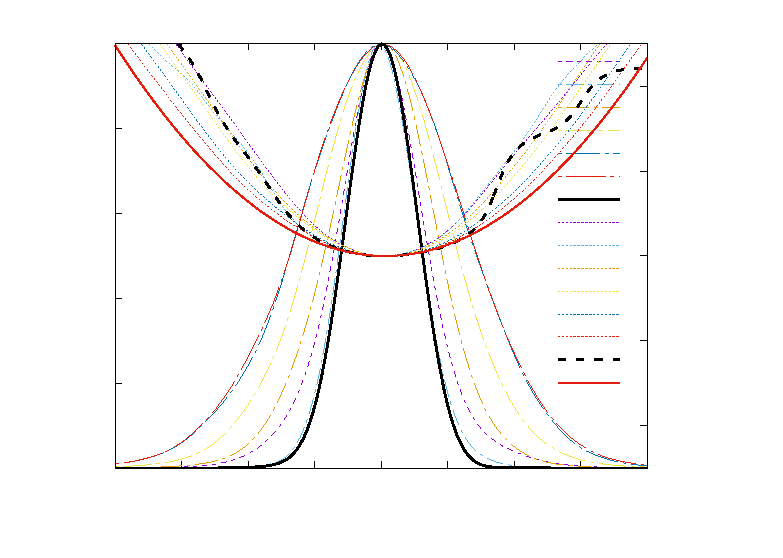
\includegraphics{temp1}}%
    \gplfronttext
  \end{picture}%
\endgroup

    \caption{blah}
    \label{fig:temp1}
\end{figure}
\begin{figure}[]
    \centering
    \input{spec1}
    \caption{blah}
    \label{fig:spec1}
\end{figure}
\begin{figure}[]
    \centering
    \input{temp2}
    \caption{blah2}
    \label{fig:temp2}
\end{figure}
\begin{figure}[]
    \centering
    % GNUPLOT: LaTeX picture with Postscript
\begingroup
  \makeatletter
  \providecommand\color[2][]{%
    \GenericError{(gnuplot) \space\space\space\@spaces}{%
      Package color not loaded in conjunction with
      terminal option `colourtext'%
    }{See the gnuplot documentation for explanation.%
    }{Either use 'blacktext' in gnuplot or load the package
      color.sty in LaTeX.}%
    \renewcommand\color[2][]{}%
  }%
  \providecommand\includegraphics[2][]{%
    \GenericError{(gnuplot) \space\space\space\@spaces}{%
      Package graphicx or graphics not loaded%
    }{See the gnuplot documentation for explanation.%
    }{The gnuplot epslatex terminal needs graphicx.sty or graphics.sty.}%
    \renewcommand\includegraphics[2][]{}%
  }%
  \providecommand\rotatebox[2]{#2}%
  \@ifundefined{ifGPcolor}{%
    \newif\ifGPcolor
    \GPcolortrue
  }{}%
  \@ifundefined{ifGPblacktext}{%
    \newif\ifGPblacktext
    \GPblacktexttrue
  }{}%
  % define a \g@addto@macro without @ in the name:
  \let\gplgaddtomacro\g@addto@macro
  % define empty templates for all commands taking text:
  \gdef\gplbacktext{}%
  \gdef\gplfronttext{}%
  \makeatother
  \ifGPblacktext
    % no textcolor at all
    \def\colorrgb#1{}%
    \def\colorgray#1{}%
  \else
    % gray or color?
    \ifGPcolor
      \def\colorrgb#1{\color[rgb]{#1}}%
      \def\colorgray#1{\color[gray]{#1}}%
      \expandafter\def\csname LTw\endcsname{\color{white}}%
      \expandafter\def\csname LTb\endcsname{\color{black}}%
      \expandafter\def\csname LTa\endcsname{\color{black}}%
      \expandafter\def\csname LT0\endcsname{\color[rgb]{1,0,0}}%
      \expandafter\def\csname LT1\endcsname{\color[rgb]{0,1,0}}%
      \expandafter\def\csname LT2\endcsname{\color[rgb]{0,0,1}}%
      \expandafter\def\csname LT3\endcsname{\color[rgb]{1,0,1}}%
      \expandafter\def\csname LT4\endcsname{\color[rgb]{0,1,1}}%
      \expandafter\def\csname LT5\endcsname{\color[rgb]{1,1,0}}%
      \expandafter\def\csname LT6\endcsname{\color[rgb]{0,0,0}}%
      \expandafter\def\csname LT7\endcsname{\color[rgb]{1,0.3,0}}%
      \expandafter\def\csname LT8\endcsname{\color[rgb]{0.5,0.5,0.5}}%
    \else
      % gray
      \def\colorrgb#1{\color{black}}%
      \def\colorgray#1{\color[gray]{#1}}%
      \expandafter\def\csname LTw\endcsname{\color{white}}%
      \expandafter\def\csname LTb\endcsname{\color{black}}%
      \expandafter\def\csname LTa\endcsname{\color{black}}%
      \expandafter\def\csname LT0\endcsname{\color{black}}%
      \expandafter\def\csname LT1\endcsname{\color{black}}%
      \expandafter\def\csname LT2\endcsname{\color{black}}%
      \expandafter\def\csname LT3\endcsname{\color{black}}%
      \expandafter\def\csname LT4\endcsname{\color{black}}%
      \expandafter\def\csname LT5\endcsname{\color{black}}%
      \expandafter\def\csname LT6\endcsname{\color{black}}%
      \expandafter\def\csname LT7\endcsname{\color{black}}%
      \expandafter\def\csname LT8\endcsname{\color{black}}%
    \fi
  \fi
    \setlength{\unitlength}{0.0500bp}%
    \ifx\gptboxheight\undefined%
      \newlength{\gptboxheight}%
      \newlength{\gptboxwidth}%
      \newsavebox{\gptboxtext}%
    \fi%
    \setlength{\fboxrule}{0.5pt}%
    \setlength{\fboxsep}{1pt}%
\begin{picture}(7200.00,5040.00)%
    \gplgaddtomacro\gplbacktext{%
      \csname LTb\endcsname%
      \put(814,704){\makebox(0,0)[r]{\strut{}$0$}}%
      \put(814,1518){\makebox(0,0)[r]{\strut{}$0.2$}}%
      \put(814,2332){\makebox(0,0)[r]{\strut{}$0.4$}}%
      \put(814,3147){\makebox(0,0)[r]{\strut{}$0.6$}}%
      \put(814,3961){\makebox(0,0)[r]{\strut{}$0.8$}}%
      \put(814,4775){\makebox(0,0)[r]{\strut{}$1$}}%
      \put(1457,484){\makebox(0,0){\strut{}$760$}}%
      \put(2479,484){\makebox(0,0){\strut{}$780$}}%
      \put(3501,484){\makebox(0,0){\strut{}$800$}}%
      \put(4522,484){\makebox(0,0){\strut{}$820$}}%
      \put(5544,484){\makebox(0,0){\strut{}$840$}}%
      \put(6187,1111){\makebox(0,0)[l]{\strut{}$-4$}}%
      \put(6187,1925){\makebox(0,0)[l]{\strut{}$-2$}}%
      \put(6187,2740){\makebox(0,0)[l]{\strut{}$0$}}%
      \put(6187,3554){\makebox(0,0)[l]{\strut{}$2$}}%
      \put(6187,4368){\makebox(0,0)[l]{\strut{}$4$}}%
    }%
    \gplgaddtomacro\gplfronttext{%
      \csname LTb\endcsname%
      \put(176,2739){\rotatebox{-270}{\makebox(0,0){\strut{}Spektrale Intensität $S$}}}%
      \put(6692,2739){\rotatebox{-270}{\makebox(0,0){\strut{}Phase $\Phi$ [rad]}}}%
      \put(3500,154){\makebox(0,0){\strut{}Wellenlänge $\lambda$ [nm]}}%
      \csname LTb\endcsname%
      \put(5068,4602){\makebox(0,0)[r]{\strut{}\tiny$S:0.95\;\text{nm}$}}%
      \csname LTb\endcsname%
      \put(5068,4382){\makebox(0,0)[r]{\strut{}\tiny$S:1.45\;\text{nm}$}}%
      \csname LTb\endcsname%
      \put(5068,4162){\makebox(0,0)[r]{\strut{}\tiny$S:1.95\;\text{nm}$}}%
      \csname LTb\endcsname%
      \put(5068,3942){\makebox(0,0)[r]{\strut{}\tiny$S:2.45\;\text{nm}$}}%
      \csname LTb\endcsname%
      \put(5068,3722){\makebox(0,0)[r]{\strut{}\tiny$S:2.84\;\text{nm}$}}%
      \csname LTb\endcsname%
      \put(5068,3502){\makebox(0,0)[r]{\strut{}\tiny$S:2.84\;\text{nm (opt)}$}}%
      \csname LTb\endcsname%
      \put(5068,3282){\makebox(0,0)[r]{\strut{}\tiny$\Phi:0.95\;\text{nm}$}}%
      \csname LTb\endcsname%
      \put(5068,3062){\makebox(0,0)[r]{\strut{}\tiny$\Phi:1.45\;\text{nm}$}}%
      \csname LTb\endcsname%
      \put(5068,2842){\makebox(0,0)[r]{\strut{}\tiny$\Phi:1.95\;\text{nm}$}}%
      \csname LTb\endcsname%
      \put(5068,2622){\makebox(0,0)[r]{\strut{}\tiny$\Phi:2.45\;\text{nm}$}}%
      \csname LTb\endcsname%
      \put(5068,2402){\makebox(0,0)[r]{\strut{}\tiny$\Phi:2.84\;\text{nm}$}}%
      \csname LTb\endcsname%
      \put(5068,2182){\makebox(0,0)[r]{\strut{}\tiny$\Phi:2.84\;\text{nm (opt)}$}}%
      \csname LTb\endcsname%
      \put(5068,1962){\makebox(0,0)[r]{\strut{}fit}}%
    }%
    \gplbacktext
    \put(0,0){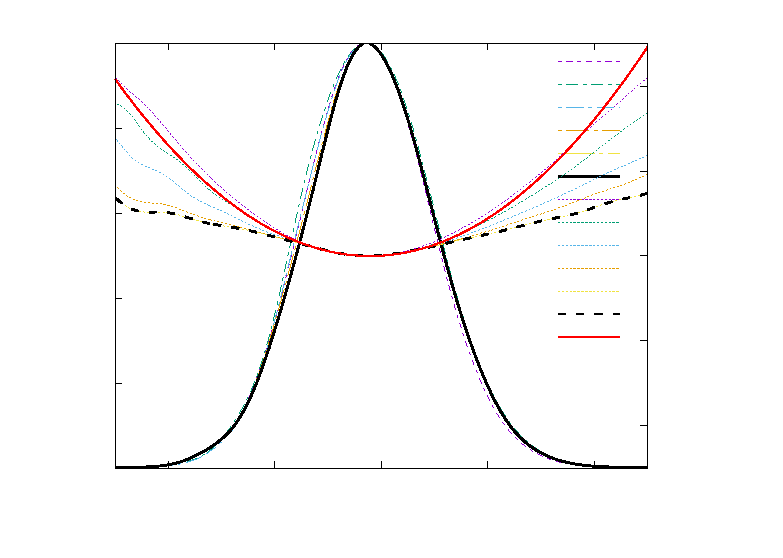
\includegraphics{spec2}}%
    \gplfronttext
  \end{picture}%
\endgroup

    \caption{blah2}
    \label{fig:spec2}
\end{figure}
\subsection{Glasfenster}
\subsection{Spatial Chirp und Pulse Front Tilt}
Der räumliche Chirp, welcher von der Quick-Frog Software gemessen wurde, ist
zusammen mit dem Puls Front tilt in \cref{tab:pft} aufgetragen. Für die Messung
ohne optische Elemente wurden ebenfalls beide Werte zum Vergleich eingetragen. 
Da von jedem Element höchstens zwei Datenpunkte vorhanden sind, wurde auf einen
Plot verzichtet. Man sieht, dass auch ohne optisches Element sowohl der PFT als
auch der räumliche Chirp nicht null sind. Deswegen ist in \cref{fig:pcpft}
beides für verschiedene Prismeneinschübe, aber ohne optisches Element
aufgetragen. Man erkennt, dass der räumliche Chirp mit steigendem
Prismeneinschub geringer wird, während der PFT wächst. Fehler wurden von der Analysesoftware nicht berechnet, aber man
kann die Schwankungen der Messwerte größer als den Messfehler des Instrumentes
annehmen.
\begin{figure}[]
    \begin{center}
        \input{pcpft.tex}
    \end{center}
    \caption{Puls Front Tilt und Spatial Chirp der Prismenkompressorausmessung
    in Abhängigkeit der Insertion.}
    \label{fig:pcpft}
\end{figure}

\begin{table}
    \centering
    \begin{tabular}[]{|c||c|c||c|c|}
        \hline
        Objekt&\multicolumn{2}{|c||}{Spatial Chirp [$10^{-5}\Delta\lambda/\Delta x$]}&\multicolumn{2}{|c|}{Pulse front tilt [$\text{fs}/\text{mm}$]}\\\hline
         &unkompensiert&kompensiert&unkompensiert&kompensiert\\ 
        \hline
        Nur PC&$-7$&-&$-8.38$&-\\\hline
        5 mm BK7&$-30$&$-5$&$-8.52$&$-8.80$\\\hline
        10 mm BK7&$-59$&$2760$&$-8.6$&$-9.80$\\\hline
        5 mm MgF2&$-20$&$-5$&$-8.59$&$-9.01$\\\hline
        5 mm BK7 $+30^\circ$&$-28$&$0.07$&$-6.59$&$-7.86$\\\hline
        5 mm BK7 $.30^\circ$&$-31$&$-8$&$-8.44$&$-8.69$\\\hline
        BK7 Keil (wedge)&$-11$&$11$&$-15.87$&$-15.1$\\\hline
        longpass&$-90$&$-44$&$-7.06$&$-8.08$\\\hline
    \end{tabular}
    \caption{Von Quick Frog gemessener räumlicher Chirp und Puls Front Tilt,
    jeweils in optimaler (unkompensierter) Prismenkonfiguration und mit
    Kompensierung für verschiedene optische Elemente.}
    \label{tab:pft}
\end{table}
\subsection{Langpassfilter}
Für den Langpassfilter sind Intensität und Spektrum jeweils in
\cref{fig:long1,fig:long2} zusammen mit den zugehörigen Phasen sowohl in
optimaler als auch in komprensierter PC-Konfiguration aufgetragen.
Ebenfalls aufgetragen ist Intensität und Spektrum inklusive Phase der Messung
ohne Langpassfilter bei optimaler Prismenkonfiguration. Die zugehörigen
Pulsdauern und Bandbreiten sind in Tabelle \cref{tab:long} zusammengefasst.
Zum Vergleich ist für die gemessene Bandbreite der Langpass-Messung mithilfe
vom Zeit-Bandprodukt \cref{eq:bandprodeasy} die resultierende Pulsdauer eines
fourierlimitierten Pulses berechnet worden.


\begin{table}
    \centering
    \begin{tabular}[]{|c||c|c|c|c|}
        \hline
        Messung&$\tau$ [fs]&$\Delta\lambda$ [nm]&$\lambda_0$ [nm]&FWHM Zeit-Bandprodukt\\\hline
        Ohne LP (opt)&24.6&45.3&793.9&0.533\\\hline
        Langpass (opt)&56.4&34.9&784.3&0.958\\\hline
        Langpass (komp)&37.4&38.6&784.3&0.702\\\hline\hline
        Theorie &25.9&34.9&784.3&0.441\\\hline

    \end{tabular}
    \caption{Pulsdauern, Bandbreiten, Trägerwellenlängen, sowie das
    Zeit-Bandprodukt der Messungen ohne und mit Langpassfilter. Für die opt.
Langpass-Messung wurde die fourierlimitierte Pulsdauer berechnet. }
    \label{tab:long}
\end{table}


\begin{figure}[]
    \begin{center}
        % GNUPLOT: LaTeX picture with Postscript
\begingroup
  \makeatletter
  \providecommand\color[2][]{%
    \GenericError{(gnuplot) \space\space\space\@spaces}{%
      Package color not loaded in conjunction with
      terminal option `colourtext'%
    }{See the gnuplot documentation for explanation.%
    }{Either use 'blacktext' in gnuplot or load the package
      color.sty in LaTeX.}%
    \renewcommand\color[2][]{}%
  }%
  \providecommand\includegraphics[2][]{%
    \GenericError{(gnuplot) \space\space\space\@spaces}{%
      Package graphicx or graphics not loaded%
    }{See the gnuplot documentation for explanation.%
    }{The gnuplot epslatex terminal needs graphicx.sty or graphics.sty.}%
    \renewcommand\includegraphics[2][]{}%
  }%
  \providecommand\rotatebox[2]{#2}%
  \@ifundefined{ifGPcolor}{%
    \newif\ifGPcolor
    \GPcolortrue
  }{}%
  \@ifundefined{ifGPblacktext}{%
    \newif\ifGPblacktext
    \GPblacktexttrue
  }{}%
  % define a \g@addto@macro without @ in the name:
  \let\gplgaddtomacro\g@addto@macro
  % define empty templates for all commands taking text:
  \gdef\gplbacktext{}%
  \gdef\gplfronttext{}%
  \makeatother
  \ifGPblacktext
    % no textcolor at all
    \def\colorrgb#1{}%
    \def\colorgray#1{}%
  \else
    % gray or color?
    \ifGPcolor
      \def\colorrgb#1{\color[rgb]{#1}}%
      \def\colorgray#1{\color[gray]{#1}}%
      \expandafter\def\csname LTw\endcsname{\color{white}}%
      \expandafter\def\csname LTb\endcsname{\color{black}}%
      \expandafter\def\csname LTa\endcsname{\color{black}}%
      \expandafter\def\csname LT0\endcsname{\color[rgb]{1,0,0}}%
      \expandafter\def\csname LT1\endcsname{\color[rgb]{0,1,0}}%
      \expandafter\def\csname LT2\endcsname{\color[rgb]{0,0,1}}%
      \expandafter\def\csname LT3\endcsname{\color[rgb]{1,0,1}}%
      \expandafter\def\csname LT4\endcsname{\color[rgb]{0,1,1}}%
      \expandafter\def\csname LT5\endcsname{\color[rgb]{1,1,0}}%
      \expandafter\def\csname LT6\endcsname{\color[rgb]{0,0,0}}%
      \expandafter\def\csname LT7\endcsname{\color[rgb]{1,0.3,0}}%
      \expandafter\def\csname LT8\endcsname{\color[rgb]{0.5,0.5,0.5}}%
    \else
      % gray
      \def\colorrgb#1{\color{black}}%
      \def\colorgray#1{\color[gray]{#1}}%
      \expandafter\def\csname LTw\endcsname{\color{white}}%
      \expandafter\def\csname LTb\endcsname{\color{black}}%
      \expandafter\def\csname LTa\endcsname{\color{black}}%
      \expandafter\def\csname LT0\endcsname{\color{black}}%
      \expandafter\def\csname LT1\endcsname{\color{black}}%
      \expandafter\def\csname LT2\endcsname{\color{black}}%
      \expandafter\def\csname LT3\endcsname{\color{black}}%
      \expandafter\def\csname LT4\endcsname{\color{black}}%
      \expandafter\def\csname LT5\endcsname{\color{black}}%
      \expandafter\def\csname LT6\endcsname{\color{black}}%
      \expandafter\def\csname LT7\endcsname{\color{black}}%
      \expandafter\def\csname LT8\endcsname{\color{black}}%
    \fi
  \fi
  \setlength{\unitlength}{0.0500bp}%
  \begin{picture}(7200.00,5040.00)%
    \gplgaddtomacro\gplbacktext{%
      \csname LTb\endcsname%
      \put(946,704){\makebox(0,0)[r]{\strut{} 0}}%
      \put(946,1518){\makebox(0,0)[r]{\strut{} 0.2}}%
      \put(946,2332){\makebox(0,0)[r]{\strut{} 0.4}}%
      \put(946,3147){\makebox(0,0)[r]{\strut{} 0.6}}%
      \put(946,3961){\makebox(0,0)[r]{\strut{} 0.8}}%
      \put(946,4775){\makebox(0,0)[r]{\strut{} 1}}%
      \put(1078,484){\makebox(0,0){\strut{}-80}}%
      \put(1700,484){\makebox(0,0){\strut{}-60}}%
      \put(2322,484){\makebox(0,0){\strut{}-40}}%
      \put(2944,484){\makebox(0,0){\strut{}-20}}%
      \put(3567,484){\makebox(0,0){\strut{} 0}}%
      \put(4189,484){\makebox(0,0){\strut{} 20}}%
      \put(4811,484){\makebox(0,0){\strut{} 40}}%
      \put(5433,484){\makebox(0,0){\strut{} 60}}%
      \put(6055,484){\makebox(0,0){\strut{} 80}}%
      \put(6187,1111){\makebox(0,0)[l]{\strut{}-4}}%
      \put(6187,1925){\makebox(0,0)[l]{\strut{}-2}}%
      \put(6187,2740){\makebox(0,0)[l]{\strut{} 0}}%
      \put(6187,3554){\makebox(0,0)[l]{\strut{} 2}}%
      \put(6187,4368){\makebox(0,0)[l]{\strut{} 4}}%
      \put(176,2739){\rotatebox{-270}{\makebox(0,0){\strut{}Intensität $I$}}}%
      \put(6692,2739){\rotatebox{-270}{\makebox(0,0){\strut{}Phase $\Phi$ [rad]}}}%
      \put(3566,154){\makebox(0,0){\strut{}Zeit $t$ [fs]}}%
    }%
    \gplgaddtomacro\gplfronttext{%
      \csname LTb\endcsname%
      \put(5068,4602){\makebox(0,0)[r]{\strut{}$I$ LP (opt)}}%
      \csname LTb\endcsname%
      \put(5068,4382){\makebox(0,0)[r]{\strut{}$\Phi$ LP (opt)}}%
      \csname LTb\endcsname%
      \put(5068,4162){\makebox(0,0)[r]{\strut{}$I$ LP (komp)}}%
      \csname LTb\endcsname%
      \put(5068,3942){\makebox(0,0)[r]{\strut{}$\Phi$ LP (komp)}}%
      \csname LTb\endcsname%
      \put(5068,3722){\makebox(0,0)[r]{\strut{}$I$ ohne LP}}%
      \csname LTb\endcsname%
      \put(5068,3502){\makebox(0,0)[r]{\strut{}$\Phi$ ohne LP}}%
    }%
    \gplbacktext
    \put(0,0){\includegraphics{longpass}}%
    \gplfronttext
  \end{picture}%
\endgroup

    \end{center}
    \caption{Intensität bei optimaler Prismenkonfiguration (opt) ohne
    Langpassfilter und bei
    eingesetztem Langpassfilter unkompensiert und kompensiert.}
    \label{fig:long1}
\end{figure}

\begin{figure}[]
    \begin{center}
        % GNUPLOT: LaTeX picture with Postscript
\begingroup
  \makeatletter
  \providecommand\color[2][]{%
    \GenericError{(gnuplot) \space\space\space\@spaces}{%
      Package color not loaded in conjunction with
      terminal option `colourtext'%
    }{See the gnuplot documentation for explanation.%
    }{Either use 'blacktext' in gnuplot or load the package
      color.sty in LaTeX.}%
    \renewcommand\color[2][]{}%
  }%
  \providecommand\includegraphics[2][]{%
    \GenericError{(gnuplot) \space\space\space\@spaces}{%
      Package graphicx or graphics not loaded%
    }{See the gnuplot documentation for explanation.%
    }{The gnuplot epslatex terminal needs graphicx.sty or graphics.sty.}%
    \renewcommand\includegraphics[2][]{}%
  }%
  \providecommand\rotatebox[2]{#2}%
  \@ifundefined{ifGPcolor}{%
    \newif\ifGPcolor
    \GPcolortrue
  }{}%
  \@ifundefined{ifGPblacktext}{%
    \newif\ifGPblacktext
    \GPblacktexttrue
  }{}%
  % define a \g@addto@macro without @ in the name:
  \let\gplgaddtomacro\g@addto@macro
  % define empty templates for all commands taking text:
  \gdef\gplbacktext{}%
  \gdef\gplfronttext{}%
  \makeatother
  \ifGPblacktext
    % no textcolor at all
    \def\colorrgb#1{}%
    \def\colorgray#1{}%
  \else
    % gray or color?
    \ifGPcolor
      \def\colorrgb#1{\color[rgb]{#1}}%
      \def\colorgray#1{\color[gray]{#1}}%
      \expandafter\def\csname LTw\endcsname{\color{white}}%
      \expandafter\def\csname LTb\endcsname{\color{black}}%
      \expandafter\def\csname LTa\endcsname{\color{black}}%
      \expandafter\def\csname LT0\endcsname{\color[rgb]{1,0,0}}%
      \expandafter\def\csname LT1\endcsname{\color[rgb]{0,1,0}}%
      \expandafter\def\csname LT2\endcsname{\color[rgb]{0,0,1}}%
      \expandafter\def\csname LT3\endcsname{\color[rgb]{1,0,1}}%
      \expandafter\def\csname LT4\endcsname{\color[rgb]{0,1,1}}%
      \expandafter\def\csname LT5\endcsname{\color[rgb]{1,1,0}}%
      \expandafter\def\csname LT6\endcsname{\color[rgb]{0,0,0}}%
      \expandafter\def\csname LT7\endcsname{\color[rgb]{1,0.3,0}}%
      \expandafter\def\csname LT8\endcsname{\color[rgb]{0.5,0.5,0.5}}%
    \else
      % gray
      \def\colorrgb#1{\color{black}}%
      \def\colorgray#1{\color[gray]{#1}}%
      \expandafter\def\csname LTw\endcsname{\color{white}}%
      \expandafter\def\csname LTb\endcsname{\color{black}}%
      \expandafter\def\csname LTa\endcsname{\color{black}}%
      \expandafter\def\csname LT0\endcsname{\color{black}}%
      \expandafter\def\csname LT1\endcsname{\color{black}}%
      \expandafter\def\csname LT2\endcsname{\color{black}}%
      \expandafter\def\csname LT3\endcsname{\color{black}}%
      \expandafter\def\csname LT4\endcsname{\color{black}}%
      \expandafter\def\csname LT5\endcsname{\color{black}}%
      \expandafter\def\csname LT6\endcsname{\color{black}}%
      \expandafter\def\csname LT7\endcsname{\color{black}}%
      \expandafter\def\csname LT8\endcsname{\color{black}}%
    \fi
  \fi
  \setlength{\unitlength}{0.0500bp}%
  \begin{picture}(7200.00,5040.00)%
    \gplgaddtomacro\gplbacktext{%
      \csname LTb\endcsname%
      \put(946,704){\makebox(0,0)[r]{\strut{} 0}}%
      \put(946,1518){\makebox(0,0)[r]{\strut{} 0.2}}%
      \put(946,2332){\makebox(0,0)[r]{\strut{} 0.4}}%
      \put(946,3147){\makebox(0,0)[r]{\strut{} 0.6}}%
      \put(946,3961){\makebox(0,0)[r]{\strut{} 0.8}}%
      \put(946,4775){\makebox(0,0)[r]{\strut{} 1}}%
      \put(1078,484){\makebox(0,0){\strut{} 740}}%
      \put(1983,484){\makebox(0,0){\strut{} 760}}%
      \put(2888,484){\makebox(0,0){\strut{} 780}}%
      \put(3793,484){\makebox(0,0){\strut{} 800}}%
      \put(4698,484){\makebox(0,0){\strut{} 820}}%
      \put(5603,484){\makebox(0,0){\strut{} 840}}%
      \put(6187,704){\makebox(0,0)[l]{\strut{}-3}}%
      \put(6187,1383){\makebox(0,0)[l]{\strut{}-2}}%
      \put(6187,2061){\makebox(0,0)[l]{\strut{}-1}}%
      \put(6187,2740){\makebox(0,0)[l]{\strut{} 0}}%
      \put(6187,3418){\makebox(0,0)[l]{\strut{} 1}}%
      \put(6187,4097){\makebox(0,0)[l]{\strut{} 2}}%
      \put(6187,4775){\makebox(0,0)[l]{\strut{} 3}}%
      \put(176,2739){\rotatebox{-270}{\makebox(0,0){\strut{}Spektrale Intensität $S$}}}%
      \put(6692,2739){\rotatebox{-270}{\makebox(0,0){\strut{}Spektrale Phase $\varphi$ [rad]}}}%
      \put(3566,154){\makebox(0,0){\strut{}Wellenlänge $\lambda$ [nm]}}%
    }%
    \gplgaddtomacro\gplfronttext{%
      \csname LTb\endcsname%
      \put(5068,4602){\makebox(0,0)[r]{\strut{}$I$ LP (opt)}}%
      \csname LTb\endcsname%
      \put(5068,4382){\makebox(0,0)[r]{\strut{}$\varphi$ LP (opt)}}%
      \csname LTb\endcsname%
      \put(5068,4162){\makebox(0,0)[r]{\strut{}$I$ LP (komp)}}%
      \csname LTb\endcsname%
      \put(5068,3942){\makebox(0,0)[r]{\strut{}$\varphi$ LP (komp)}}%
      \csname LTb\endcsname%
      \put(5068,3722){\makebox(0,0)[r]{\strut{}$I$ ohne LP}}%
      \csname LTb\endcsname%
      \put(5068,3502){\makebox(0,0)[r]{\strut{}$\varphi$ ohne LP}}%
    }%
    \gplbacktext
    \put(0,0){\includegraphics{longpass2}}%
    \gplfronttext
  \end{picture}%
\endgroup

    \end{center}
    \caption{Spektrum bei optimaler Prismenkonfiguration (opt) ohne
    Langpassfilter und mit eingesetztem Langpassfilter, unkompensiert und
    kompensiert.}
    \label{fig:long2}
\end{figure}

\subsection{Dielektrische Spiegel}
Die Messung für Pfad 2 mit den drei dielektrischen Spiegeln ergab ein sehr
verzerrtes FROG-Trace (\cref{fig:diel}). Als vergleich ist der Trace der optimalen
Prismenkompressor-Messung in \cref{fig:opttrace} zu sehen. Aufgrund dieser
Verzerrung und da der FROG-error sehr groß ist, ist keine sinnvolle
Rekonstruktion der Pulsform möglich. Ebenso ist aus dem Spektrum keine
sinnvolle Information zu entnehmen, außer dass hier erhebliche Verzerrungen
auftreten. Die Pulsform wird von den dielektrischen Spiegeln regelrecht
zerstört. Auch eine Kompensierung mit dem Prismenkompressor war unmöglich: Die
Pulsdauer war absolut unberührt von dem Einschub des zweiten Prismas.

\begin{figure}[]
    \centering
    \includegraphics[width=0.3\textwidth]{diel.jpg}
    \caption{Experimenteller FROG trace für die Messung mit dielektrischen
    Spiegeln. Der Trace ist sehr verzerrt, wodurch keine sinnvolle
Rekonstruktion der Pulsform möglich ist. }
    \label{fig:diel}
\end{figure}
\begin{figure}[]
    \centering
    \includegraphics[width=0.3\textwidth]{opttrace.jpg}
    \caption{Experimenteller FROG trace der optimalen Prismenkompressormessung.}
    \label{fig:opttrace}
\end{figure}

\subsection{Rechteckiges Spiegelpaar}
Für die Rechteckspiegel mit jeweils 5 Reflektionen zeichnet sich ein ähnliches
Bild, wie für die dielektrischen Spiegel ab. Der FROG-Trace ist verzerrt
und der FROG error ist groß ebenso sind der rekonstruierte FROG trace stark
unterschiedlich vom experimentellen. Die Ergebnisse sind in \cref{fig:chirpspiegel1}
für die unkompensierte, sowie in \cref{fig:chirpspiegel2} für die kompensierte
Messung zu sehen. Allerdings sind die Verzerrungen hier nicht so stark wie
zuvor. Die Pulsintensität, sowie das Spektrum mit Phase sind in
\cref{fig:chirptemp,fig:chirpspec} zu sehen. Man erkennt eine deutliche
Phasenfluktuation, sowie eine große Pulsbreite bei den kompensierten
Prismenkompressoreinstellungen. Die Messungen in optimaler Einstellung sind
stattdessen mit Ausnahme von einigen Einschneidungen in der Intensitätnahezu
Gaußförmig, wenn auch mit deutlich größerer Pulsdauer im Vergleich zu den 
metallischen Spiegeln.


\begin{figure}[]
    \centering
    \includegraphics[width=0.3\textwidth]{chirpsp1.jpg}
    \caption{Experimenteller FROG trace des Spiegelpaares}
    \label{fig:chirpspiegel1}
\end{figure}
\begin{figure}[]
    \centering
    \includegraphics[width=0.3\textwidth]{chirpsp2.jpg}
    \caption{Rekonstruierter FROG trace des Spiegelpaares}
    \label{fig:chirpspiegel2}
\end{figure}
\begin{figure}[]
    \centering
    % GNUPLOT: LaTeX picture with Postscript
\begingroup
  \makeatletter
  \providecommand\color[2][]{%
    \GenericError{(gnuplot) \space\space\space\@spaces}{%
      Package color not loaded in conjunction with
      terminal option `colourtext'%
    }{See the gnuplot documentation for explanation.%
    }{Either use 'blacktext' in gnuplot or load the package
      color.sty in LaTeX.}%
    \renewcommand\color[2][]{}%
  }%
  \providecommand\includegraphics[2][]{%
    \GenericError{(gnuplot) \space\space\space\@spaces}{%
      Package graphicx or graphics not loaded%
    }{See the gnuplot documentation for explanation.%
    }{The gnuplot epslatex terminal needs graphicx.sty or graphics.sty.}%
    \renewcommand\includegraphics[2][]{}%
  }%
  \providecommand\rotatebox[2]{#2}%
  \@ifundefined{ifGPcolor}{%
    \newif\ifGPcolor
    \GPcolortrue
  }{}%
  \@ifundefined{ifGPblacktext}{%
    \newif\ifGPblacktext
    \GPblacktexttrue
  }{}%
  % define a \g@addto@macro without @ in the name:
  \let\gplgaddtomacro\g@addto@macro
  % define empty templates for all commands taking text:
  \gdef\gplbacktext{}%
  \gdef\gplfronttext{}%
  \makeatother
  \ifGPblacktext
    % no textcolor at all
    \def\colorrgb#1{}%
    \def\colorgray#1{}%
  \else
    % gray or color?
    \ifGPcolor
      \def\colorrgb#1{\color[rgb]{#1}}%
      \def\colorgray#1{\color[gray]{#1}}%
      \expandafter\def\csname LTw\endcsname{\color{white}}%
      \expandafter\def\csname LTb\endcsname{\color{black}}%
      \expandafter\def\csname LTa\endcsname{\color{black}}%
      \expandafter\def\csname LT0\endcsname{\color[rgb]{1,0,0}}%
      \expandafter\def\csname LT1\endcsname{\color[rgb]{0,1,0}}%
      \expandafter\def\csname LT2\endcsname{\color[rgb]{0,0,1}}%
      \expandafter\def\csname LT3\endcsname{\color[rgb]{1,0,1}}%
      \expandafter\def\csname LT4\endcsname{\color[rgb]{0,1,1}}%
      \expandafter\def\csname LT5\endcsname{\color[rgb]{1,1,0}}%
      \expandafter\def\csname LT6\endcsname{\color[rgb]{0,0,0}}%
      \expandafter\def\csname LT7\endcsname{\color[rgb]{1,0.3,0}}%
      \expandafter\def\csname LT8\endcsname{\color[rgb]{0.5,0.5,0.5}}%
    \else
      % gray
      \def\colorrgb#1{\color{black}}%
      \def\colorgray#1{\color[gray]{#1}}%
      \expandafter\def\csname LTw\endcsname{\color{white}}%
      \expandafter\def\csname LTb\endcsname{\color{black}}%
      \expandafter\def\csname LTa\endcsname{\color{black}}%
      \expandafter\def\csname LT0\endcsname{\color{black}}%
      \expandafter\def\csname LT1\endcsname{\color{black}}%
      \expandafter\def\csname LT2\endcsname{\color{black}}%
      \expandafter\def\csname LT3\endcsname{\color{black}}%
      \expandafter\def\csname LT4\endcsname{\color{black}}%
      \expandafter\def\csname LT5\endcsname{\color{black}}%
      \expandafter\def\csname LT6\endcsname{\color{black}}%
      \expandafter\def\csname LT7\endcsname{\color{black}}%
      \expandafter\def\csname LT8\endcsname{\color{black}}%
    \fi
  \fi
    \setlength{\unitlength}{0.0500bp}%
    \ifx\gptboxheight\undefined%
      \newlength{\gptboxheight}%
      \newlength{\gptboxwidth}%
      \newsavebox{\gptboxtext}%
    \fi%
    \setlength{\fboxrule}{0.5pt}%
    \setlength{\fboxsep}{1pt}%
\begin{picture}(7200.00,5040.00)%
    \gplgaddtomacro\gplbacktext{%
      \csname LTb\endcsname%
      \put(814,704){\makebox(0,0)[r]{\strut{}$0$}}%
      \put(814,1518){\makebox(0,0)[r]{\strut{}$0.2$}}%
      \put(814,2332){\makebox(0,0)[r]{\strut{}$0.4$}}%
      \put(814,3147){\makebox(0,0)[r]{\strut{}$0.6$}}%
      \put(814,3961){\makebox(0,0)[r]{\strut{}$0.8$}}%
      \put(814,4775){\makebox(0,0)[r]{\strut{}$1$}}%
      \put(946,484){\makebox(0,0){\strut{}$-250$}}%
      \put(1457,484){\makebox(0,0){\strut{}$-200$}}%
      \put(1968,484){\makebox(0,0){\strut{}$-150$}}%
      \put(2479,484){\makebox(0,0){\strut{}$-100$}}%
      \put(2990,484){\makebox(0,0){\strut{}$-50$}}%
      \put(3501,484){\makebox(0,0){\strut{}$0$}}%
      \put(4011,484){\makebox(0,0){\strut{}$50$}}%
      \put(4522,484){\makebox(0,0){\strut{}$100$}}%
      \put(5033,484){\makebox(0,0){\strut{}$150$}}%
      \put(5544,484){\makebox(0,0){\strut{}$200$}}%
      \put(6055,484){\makebox(0,0){\strut{}$250$}}%
      \put(6187,1111){\makebox(0,0)[l]{\strut{}$-4$}}%
      \put(6187,1925){\makebox(0,0)[l]{\strut{}$-2$}}%
      \put(6187,2740){\makebox(0,0)[l]{\strut{}$0$}}%
      \put(6187,3554){\makebox(0,0)[l]{\strut{}$2$}}%
      \put(6187,4368){\makebox(0,0)[l]{\strut{}$4$}}%
    }%
    \gplgaddtomacro\gplfronttext{%
      \csname LTb\endcsname%
      \put(176,2739){\rotatebox{-270}{\makebox(0,0){\strut{}Intensität $I$}}}%
      \put(6692,2739){\rotatebox{-270}{\makebox(0,0){\strut{}Phase $\Phi$ [rad]}}}%
      \put(3500,154){\makebox(0,0){\strut{}Zeit $t$ [fs]}}%
      \csname LTb\endcsname%
      \put(5068,4602){\makebox(0,0)[r]{\strut{}$I$ (opt)}}%
      \csname LTb\endcsname%
      \put(5068,4382){\makebox(0,0)[r]{\strut{}$\Phi$ (opt)}}%
      \csname LTb\endcsname%
      \put(5068,4162){\makebox(0,0)[r]{\strut{}$I$ (komp)}}%
      \csname LTb\endcsname%
      \put(5068,3942){\makebox(0,0)[r]{\strut{}$\Phi$ (komp)}}%
    }%
    \gplbacktext
    \put(0,0){\includegraphics{chirptemp}}%
    \gplfronttext
  \end{picture}%
\endgroup

    \caption{Experimenteller FROG trace des Spiegelpaares}
    \label{fig:chirptemp}
\end{figure}
\begin{figure}[]
    \centering
    % GNUPLOT: LaTeX picture with Postscript
\begingroup
  \makeatletter
  \providecommand\color[2][]{%
    \GenericError{(gnuplot) \space\space\space\@spaces}{%
      Package color not loaded in conjunction with
      terminal option `colourtext'%
    }{See the gnuplot documentation for explanation.%
    }{Either use 'blacktext' in gnuplot or load the package
      color.sty in LaTeX.}%
    \renewcommand\color[2][]{}%
  }%
  \providecommand\includegraphics[2][]{%
    \GenericError{(gnuplot) \space\space\space\@spaces}{%
      Package graphicx or graphics not loaded%
    }{See the gnuplot documentation for explanation.%
    }{The gnuplot epslatex terminal needs graphicx.sty or graphics.sty.}%
    \renewcommand\includegraphics[2][]{}%
  }%
  \providecommand\rotatebox[2]{#2}%
  \@ifundefined{ifGPcolor}{%
    \newif\ifGPcolor
    \GPcolortrue
  }{}%
  \@ifundefined{ifGPblacktext}{%
    \newif\ifGPblacktext
    \GPblacktexttrue
  }{}%
  % define a \g@addto@macro without @ in the name:
  \let\gplgaddtomacro\g@addto@macro
  % define empty templates for all commands taking text:
  \gdef\gplbacktext{}%
  \gdef\gplfronttext{}%
  \makeatother
  \ifGPblacktext
    % no textcolor at all
    \def\colorrgb#1{}%
    \def\colorgray#1{}%
  \else
    % gray or color?
    \ifGPcolor
      \def\colorrgb#1{\color[rgb]{#1}}%
      \def\colorgray#1{\color[gray]{#1}}%
      \expandafter\def\csname LTw\endcsname{\color{white}}%
      \expandafter\def\csname LTb\endcsname{\color{black}}%
      \expandafter\def\csname LTa\endcsname{\color{black}}%
      \expandafter\def\csname LT0\endcsname{\color[rgb]{1,0,0}}%
      \expandafter\def\csname LT1\endcsname{\color[rgb]{0,1,0}}%
      \expandafter\def\csname LT2\endcsname{\color[rgb]{0,0,1}}%
      \expandafter\def\csname LT3\endcsname{\color[rgb]{1,0,1}}%
      \expandafter\def\csname LT4\endcsname{\color[rgb]{0,1,1}}%
      \expandafter\def\csname LT5\endcsname{\color[rgb]{1,1,0}}%
      \expandafter\def\csname LT6\endcsname{\color[rgb]{0,0,0}}%
      \expandafter\def\csname LT7\endcsname{\color[rgb]{1,0.3,0}}%
      \expandafter\def\csname LT8\endcsname{\color[rgb]{0.5,0.5,0.5}}%
    \else
      % gray
      \def\colorrgb#1{\color{black}}%
      \def\colorgray#1{\color[gray]{#1}}%
      \expandafter\def\csname LTw\endcsname{\color{white}}%
      \expandafter\def\csname LTb\endcsname{\color{black}}%
      \expandafter\def\csname LTa\endcsname{\color{black}}%
      \expandafter\def\csname LT0\endcsname{\color{black}}%
      \expandafter\def\csname LT1\endcsname{\color{black}}%
      \expandafter\def\csname LT2\endcsname{\color{black}}%
      \expandafter\def\csname LT3\endcsname{\color{black}}%
      \expandafter\def\csname LT4\endcsname{\color{black}}%
      \expandafter\def\csname LT5\endcsname{\color{black}}%
      \expandafter\def\csname LT6\endcsname{\color{black}}%
      \expandafter\def\csname LT7\endcsname{\color{black}}%
      \expandafter\def\csname LT8\endcsname{\color{black}}%
    \fi
  \fi
    \setlength{\unitlength}{0.0500bp}%
    \ifx\gptboxheight\undefined%
      \newlength{\gptboxheight}%
      \newlength{\gptboxwidth}%
      \newsavebox{\gptboxtext}%
    \fi%
    \setlength{\fboxrule}{0.5pt}%
    \setlength{\fboxsep}{1pt}%
\begin{picture}(7200.00,5040.00)%
    \gplgaddtomacro\gplbacktext{%
      \csname LTb\endcsname%
      \put(814,704){\makebox(0,0)[r]{\strut{}$0$}}%
      \put(814,1518){\makebox(0,0)[r]{\strut{}$0.2$}}%
      \put(814,2332){\makebox(0,0)[r]{\strut{}$0.4$}}%
      \put(814,3147){\makebox(0,0)[r]{\strut{}$0.6$}}%
      \put(814,3961){\makebox(0,0)[r]{\strut{}$0.8$}}%
      \put(814,4775){\makebox(0,0)[r]{\strut{}$1$}}%
      \put(946,484){\makebox(0,0){\strut{}$740$}}%
      \put(1875,484){\makebox(0,0){\strut{}$760$}}%
      \put(2804,484){\makebox(0,0){\strut{}$780$}}%
      \put(3733,484){\makebox(0,0){\strut{}$800$}}%
      \put(4662,484){\makebox(0,0){\strut{}$820$}}%
      \put(5591,484){\makebox(0,0){\strut{}$840$}}%
      \put(6187,704){\makebox(0,0)[l]{\strut{}$-3$}}%
      \put(6187,1383){\makebox(0,0)[l]{\strut{}$-2$}}%
      \put(6187,2061){\makebox(0,0)[l]{\strut{}$-1$}}%
      \put(6187,2740){\makebox(0,0)[l]{\strut{}$0$}}%
      \put(6187,3418){\makebox(0,0)[l]{\strut{}$1$}}%
      \put(6187,4097){\makebox(0,0)[l]{\strut{}$2$}}%
      \put(6187,4775){\makebox(0,0)[l]{\strut{}$3$}}%
    }%
    \gplgaddtomacro\gplfronttext{%
      \csname LTb\endcsname%
      \put(176,2739){\rotatebox{-270}{\makebox(0,0){\strut{}Spektrale Intensität $S$}}}%
      \put(6692,2739){\rotatebox{-270}{\makebox(0,0){\strut{}Spektrale Phase $\varphi$ [rad]}}}%
      \put(3500,154){\makebox(0,0){\strut{}Wellenlänge $\lambda$ [nm]}}%
      \csname LTb\endcsname%
      \put(5068,4602){\makebox(0,0)[r]{\strut{}$S$ (opt)}}%
      \csname LTb\endcsname%
      \put(5068,4382){\makebox(0,0)[r]{\strut{}$\varphi$ (opt)}}%
      \csname LTb\endcsname%
      \put(5068,4162){\makebox(0,0)[r]{\strut{}$S$ (komp)}}%
      \csname LTb\endcsname%
      \put(5068,3942){\makebox(0,0)[r]{\strut{}$\varphi$ (komp)}}%
    }%
    \gplbacktext
    \put(0,0){\includegraphics{chirpspec}}%
    \gplfronttext
  \end{picture}%
\endgroup

    \caption{Rekonstruierter FROG trace des Spiegelpaares}
    \label{fig:chirpspec}
\end{figure}

\section{Diskussion}
\cite{tidecks1990current}


\bibliography{literatur}

\end{document}

